

\begin{figure}
\begin{subfigure}{.5\linewidth}
\centering

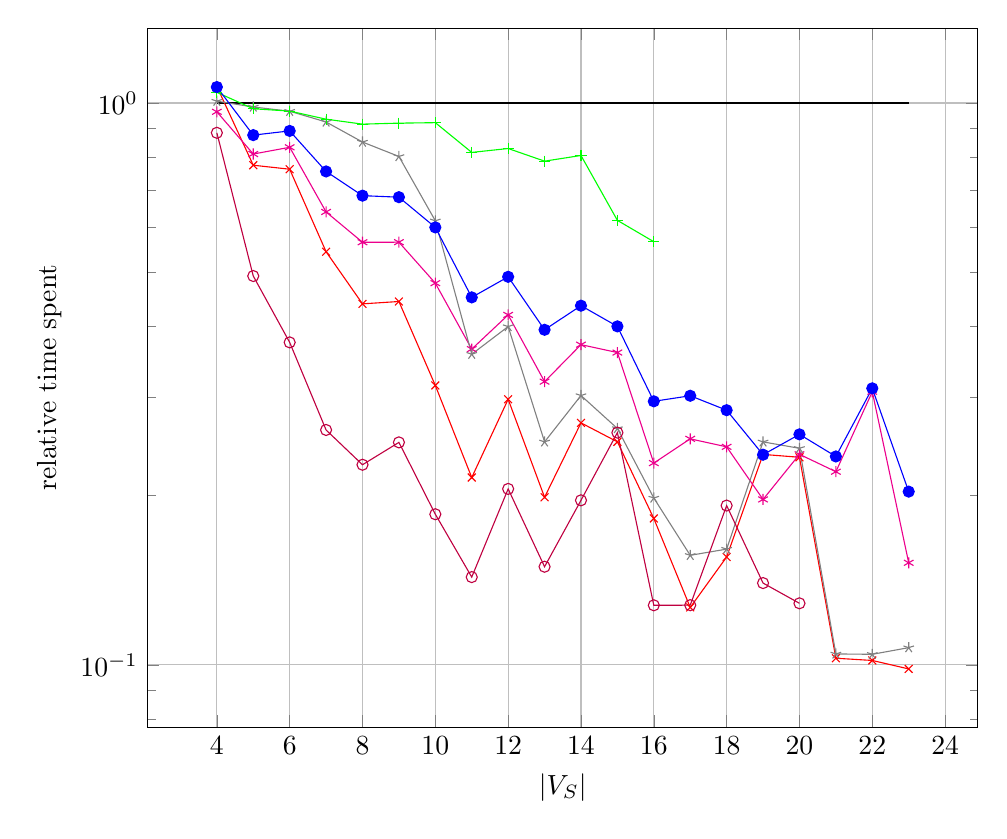
\begin{tikzpicture}
    \begin{axis}[
        xlabel=$|V_S|$,
        ylabel=relative time spent,
        ymode=log,
        legend style={at={(0.9,0.1)},anchor=south east},
        width=\textwidth,
		y tick label style={/pgf/number format/sci},
        ymajorgrids,
        xmajorgrids,		
    ]


\addplot [mark=none, black] plot coordinates {
        (4,1) (23, 1)};
%\addlegendentry{No contraction}

	
   	\addplot[
        mark=x,
        red,
    ] plot coordinates {
    (4,1.0701376596978578)
        (5,0.7750483833840601)
        (6,0.7625239659727396)
        (7,0.5435907248272545)
        (8,0.43905625641231655)
        (9,0.44333498504649627)
        (10,0.31427736006275914)
        (11,0.21549418093434788)
        (12,0.29700850327105366)
        (13,0.19875803647232598)
        (14,0.26960460127846947)
        (15,0.24943654671207566)
        (16,0.1822160520770154)
        (17,0.12652580040513978)
        (18,0.15557887314603722)
        (19,0.23690016515325316)
        (20,0.23413010848141239)
        (21,0.10274440066614124)
        (22,0.1018143796654711)
        (23,0.09833948238303787)
};
%    \addlegendentry{DFS}

\addplot[
        mark=asterisk,
        magenta,
    ] plot coordinates {
        (4,0.9646835529917239)
        (5,0.8113643330208755)
        (6,0.8340623913309159)
        (7,0.6399015712888031)
        (8,0.5651878881557018)
        (9,0.5653315538963386)
        (10,0.47794089388172367)
        (11,0.3647432871506055)
        (12,0.4196279793254562)
        (13,0.31920174684238656)
        (14,0.3714797511403636)
        (15,0.35966164286125674)
        (16,0.2286295557311787)
        (17,0.25250106787609233)
        (18,0.24436238655507947)
        (19,0.19700769848171182)
        (20,0.23697864076629702)
        (21,0.2206956999692248)
        (22,0.3062630315305542)
        (23,0.15194030658042346)
};
%    \addlegendentry{GDFS A IP}

\addplot[
        mark=star,
        gray,
    ] plot coordinates {
        (4,1.0076928820459565)
        (5,0.983901080688342)
        (6,0.9669262144955426)
        (7,0.9252245633448803)
        (8,0.8522498237398553)
        (9,0.8032759861174249)
        (10,0.6171724435688729)
        (11,0.35723830908397847)
        (12,0.4000599943535533)
        (13,0.24939686313601822)
        (14,0.3015786625876812)
        (15,0.2634252154093511)
        (16,0.19816461150852743)
        (17,0.15666932104640147)
        (18,0.16070461860726504)
        (19,0.2493749238156936)
        (20,0.24288582897080782)
        (21,0.10457106920534778)
        (22,0.10441999655858641)
        (23,0.10730037259146949)
};
%    \addlegendentry{GDFS C}

\addplot[
        mark=o,
        purple,
    ] plot coordinates {
        (4,0.8850973682092008)
        (5,0.49211719526852293)
        (6,0.3749857639782973)
        (7,0.26185344137719707)
        (8,0.22707613716934089)
        (9,0.24886610684918653)
        (10,0.18538190648139338)
        (11,0.143287178899486)
        (12,0.20567173874574307)
        (13,0.1494998841435096)
        (14,0.1962904826921925)
        (15,0.25901877438054843)
        (16,0.12764073117929187)
        (17,0.1277078372348921)
        (18,0.19211906685956734)
        (19,0.13981954023222753)
        (20,0.12868526509582714)
};
%    \addlegendentry{GDFS O IP}

\addplot[
        mark=+,
        green,
    ] plot coordinates {
        (4,1.0447200482417789)
        (5,0.9768014047219801)
        (6,0.9674489096177588)
        (7,0.9359261518821227)
        (8,0.9170755875946195)
        (9,0.9208456200850942)
        (10,0.9226483399970833)
        (11,0.8167296172561879)
        (12,0.8299040306597638)
        (13,0.7882084677764385)
        (14,0.8065343267082437)
        (15,0.6182293453860566)
        (16,0.5664050892049144)
};
%    \addlegendentry{CP}

\addplot[
        mark=*,
        blue,
    ] plot coordinates {
     (4,1.067574077798301)
        (5,0.8767234058268033)
        (6,0.8920189758885858)
        (7,0.7554709717371)
        (8,0.6841141477377559)
        (9,0.6798868705510517)
        (10,0.6006702804910036)
        (11,0.4508897423728995)
        (12,0.49054030937361914)
        (13,0.3948424128676263)
        (14,0.4358083432482373)
        (15,0.40033987136573546)
        (16,0.2944817051689707)
        (17,0.3012804658022599)
        (18,0.28397895980322047)
        (19,0.23660584413000785)
        (20,0.257186007511192)
        (21,0.2349170834392937)
        (22,0.31059677707523903)
        (23,0.2033838178427883)
};
%    \addlegendentry{K-Path}
   

    \end{axis}
    \end{tikzpicture}


\caption{$|V_T|=1\frac{1}{2}*|V_S|$}
\end{subfigure}%
\begin{subfigure}{.5\linewidth}
\centering

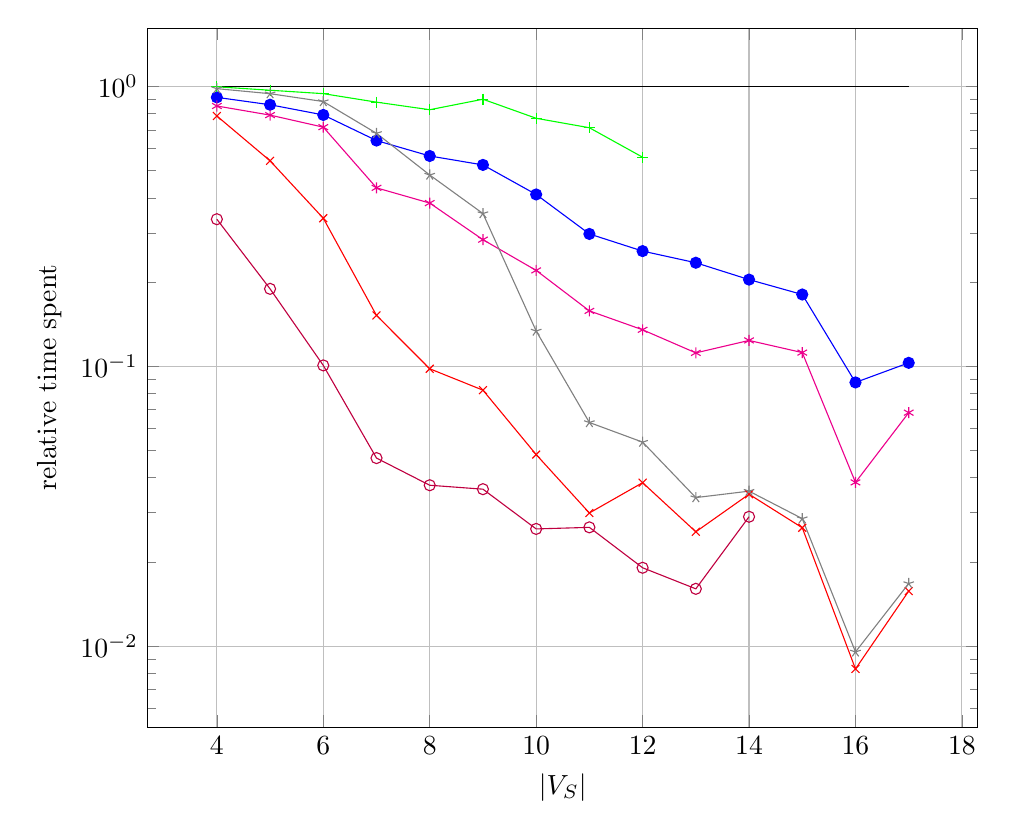
\begin{tikzpicture}
    \begin{axis}[
        xlabel=$|V_S|$,
        ylabel=relative time spent,
        ymode=log,
        legend style={at={(0.9,0.1)},anchor=south east},
        width=\textwidth,
		y tick label style={/pgf/number format/sci},
        ymajorgrids,
        xmajorgrids,		
    ]


\addplot [mark=none, black] plot coordinates {
        (4,1) (17, 1)};
%\addlegendentry{No contraction}

	
\addplot[
        mark=*,
        blue,
    ] plot coordinates {
        (4,0.9144351873245234)
        (5,0.8604827367991432)
        (6,0.7913807944471791)
        (7,0.6408747361080422)
        (8,0.5644869931387801)
        (9,0.5244957804593064)
        (10,0.41127045927825046)
        (11,0.29721708517427003)
        (12,0.25807846072204743)
        (13,0.23450003716530787)
        (14,0.20415508777162117)
        (15,0.1806016795323983)
        (16,0.08759221597847955)
        (17,0.1029272468937503)
 
};
 %   \addlegendentry{K-Path}
    
    
    
    \addplot[
        mark=asterisk,
        magenta,
    ] plot coordinates {
        (4,0.8517306816100106)
        (5,0.7903396576378922)
        (6,0.715605937049185)
        (7,0.43437312425655195)
        (8,0.3831879607610557)
        (9,0.28351535934948463)
        (10,0.22018179650022743)
        (11,0.15781373311519534)
        (12,0.13507446584999497)
        (13,0.11170957349041666)
        (14,0.12375046702003706)
        (15,0.11197654989350668)
        (16,0.03848467373571145)
        (17,0.06830118707399156)
   
};
 %   \addlegendentry{GDFS A IP}
    
    
    \addplot[
        mark=x,
        red,
    ] plot coordinates {
        (4,0.7846872619727697)
        (5,0.5424712735363988)
        (6,0.3382315124928066)
        (7,0.15200192583513225)
        (8,0.09801750480507616)
        (9,0.08219886549722584)
        (10,0.04838061481784399)
        (11,0.0299220609181214)
        (12,0.03839698220605832)
        (13,0.025633258543015524)
        (14,0.034913185288842526)
        (15,0.026500220293965936)
        (16,0.008292853704258583)
        (17,0.01573584213744253)
      
};
%    \addlegendentry{DFS}

\addplot[
        mark=+,
        green,
    ] plot coordinates {
        (4,0.9973998175073646)
        (5,0.9695932261369062)
        (6,0.9426984145150554)
        (7,0.8790360004733055)
        (8,0.8258952335172475)
        (9,0.9003838932139886)
        (10,0.7698527105174667)
        (11,0.7122224617463608)
        (12,0.5588810419114151)
     
};
%    \addlegendentry{CP}

\addplot[
        mark=o,
        purple,
    ] plot coordinates {
        (4,0.33554458139095233)
        (5,0.18918210118040157)
        (6,0.1007740374152106)
        (7,0.04700465229827888)
        (8,0.03759650462559647)
        (9,0.036396221646248145)
        (10,0.02624491328700947)
        (11,0.02658394145808671)
        (12,0.019067253573874218)
        (13,0.016032335955180207)
        (14,0.029010454773618948)
     
};
%    \addlegendentry{GDFS O IP}

\addplot[
        mark=star,
        gray,
    ] plot coordinates {
        (4,0.9823157213858835)
        (5,0.9423930396188176)
        (6,0.8834397867884509)
        (7,0.6802397523203553)
        (8,0.4827313559711965)
        (9,0.35157298039088664)
        (10,0.13375480538418397)
        (11,0.06300868845254717)
        (12,0.05360184520525508)
        (13,0.03396322326203567)
        (14,0.035813414894332325)
        (15,0.02857019872219001)
        (16,0.00953880632335426)
        (17,0.016748489489447828)
      
};
%    \addlegendentry{GDFS C}


    \end{axis}
    \end{tikzpicture}

\caption{$|V_T|=3*|V_S|$}
\end{subfigure}\\[1ex]
\begin{subfigure}{0.5\linewidth}
\centering

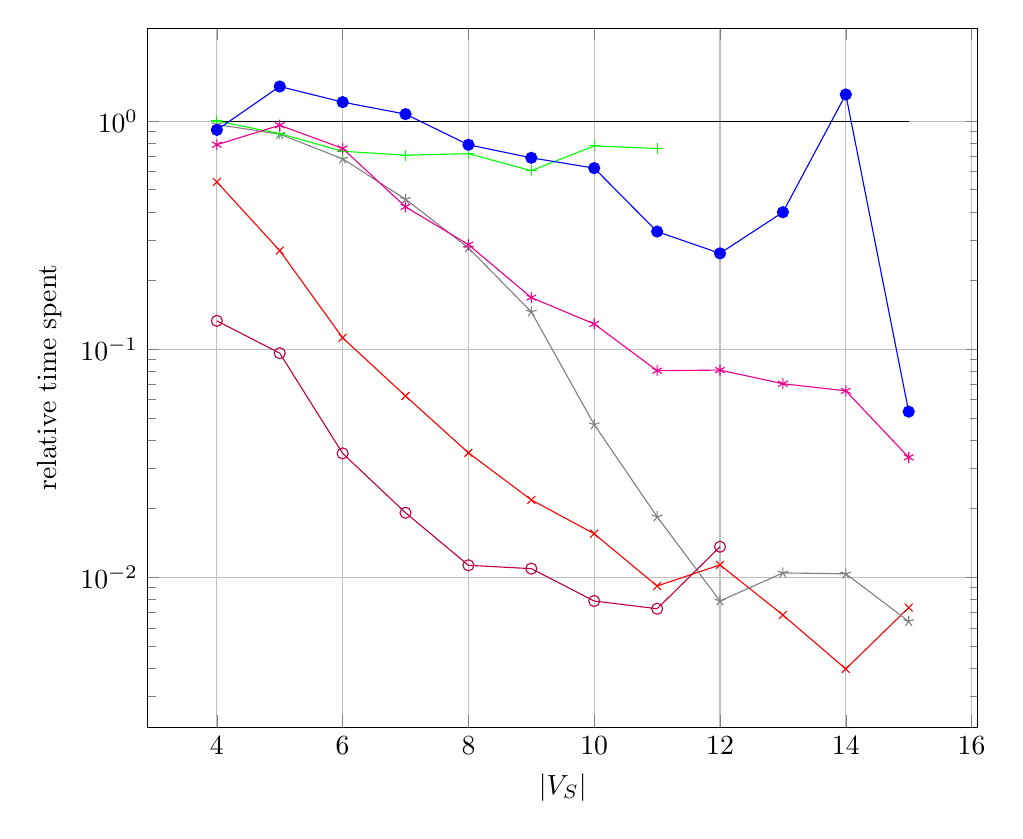
\begin{tikzpicture}
    \begin{axis}[
        xlabel=$|V_S|$,
        ylabel=relative time spent,
        ymode=log,
        legend style={at={(0.9,0.1)},anchor=south east},
        width=\textwidth,
		y tick label style={/pgf/number format/sci},
        ymajorgrids,
        xmajorgrids,		
    ]


\addplot [mark=none, black] plot coordinates {
        (4,1) (15, 1)};
%\addlegendentry{No contraction}

	

\addplot[
        mark=x,
        red,
    ] plot coordinates {
        (4,0.5411179697032152)
        (5,0.2704930524379897)
        (6,0.11213082723419009)
        (7,0.06232599283874147)
        (8,0.035108158298212004)
        (9,0.021832359512569)
        (10,0.01551029778400324)
        (11,0.009148749886694655)
        (12,0.011322643138557083)
        (13,0.00682563520131426)
        (14,0.00396036408059703)
        (15,0.007353396321165447)      
};
%    \addlegendentry{DFS}

\addplot[
        mark=star,
        gray,
    ] plot coordinates {
        (4,0.9666239578598108)
        (5,0.8762877842065461)
        (6,0.683608559713269)
        (7,0.4546873986370473)
        (8,0.27810210244800715)
        (9,0.14573574757374422)
        (10,0.04669051634035179)
        (11,0.01841463663053203)
        (12,0.007868256524489591)
        (13,0.010439288181501596)
        (14,0.010347609542544794)
        (15,0.0064051732486205175)
       
};
%    \addlegendentry{GDFS C}


\addplot[
        mark=+,
        green,
    ] plot coordinates {
        (4,1.0015024125207466)
        (5,0.8816514833540374)
        (6,0.7375927572761795)
        (7,0.7090274940418195)
        (8,0.7199742258925761)
        (9,0.6062582608534516)
        (10,0.7786554757622911)
        (11,0.759062007941154)
       
};
%    \addlegendentry{CP}


\addplot[
        mark=o,
        purple,
    ] plot coordinates {
        (4,0.13311802967905184)
        (5,0.09603338861901747)
        (6,0.034918336842012156)
        (7,0.01917346709192102)
        (8,0.011276855984884832)
        (9,0.01090036189935871)
        (10,0.007862390877023315)
        (11,0.007272947391639492)
        (12,0.01359730670398279)
      
};
%    \addlegendentry{GDFS O IP}

\addplot[
        mark=asterisk,
        magenta,
    ] plot coordinates {
        (4,0.788292323592923)
        (5,0.9590318454161153)
        (6,0.7592089649215885)
        (7,0.4208192590438211)
        (8,0.2873834837908332)
        (9,0.16830317135597236)
        (10,0.12898635225142394)
        (11,0.08047180918507638)
        (12,0.0809381779051798)
        (13,0.07055502127681917)
        (14,0.06566668124638324)
        (15,0.03353747138923799)
       
};
%    \addlegendentry{GDFS A IP}


\addplot[
        mark=*,
        blue,
    ] plot coordinates {
        (4,0.9150693631849841)
        (5,1.4188871468301367)
        (6,1.211562728934971)
        (7,1.0731297341357748)
        (8,0.7875188029533118)
        (9,0.6903542117220096)
        (10,0.62219988843212)
        (11,0.3278805811742973)
        (12,0.2630839875412322)
        (13,0.3986393081117181)
        (14,1.3090500221932537)
        (15,0.053211168492635234)
      
};
%    \addlegendentry{K-Path}
	
    \end{axis}
    \end{tikzpicture}

\caption{$|V_T|=5*|V_S|$}
\end{subfigure}
\begin{subfigure} {0.5\linewidth}
\centering

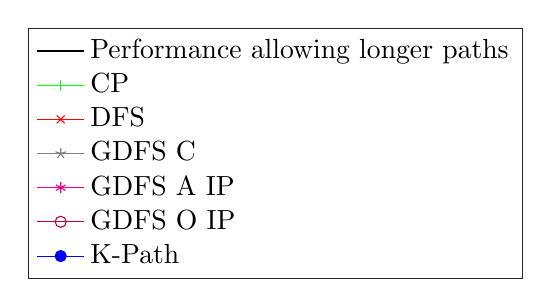
\begin{tikzpicture} 
    \begin{axis}[%
    hide axis,
    xmin=10,
    xmax=50,
    ymin=0,
    ymax=0.4,
    legend style={draw=white!15!black,legend cell align=left}
    ]
	\addlegendimage{black}
    \addlegendentry{Performance allowing longer paths}; 
     
    \addlegendimage{green, mark=+}
    \addlegendentry{CP};
    
    \addlegendimage{red, mark=x}
    \addlegendentry{DFS};
    
    \addlegendimage{gray, mark=star}
    \addlegendentry{GDFS C};
    
    \addlegendimage{magenta, mark=asterisk}
    \addlegendentry{GDFS A IP};
    
    \addlegendimage{purple, mark=o}
    \addlegendentry{GDFS O IP};
    
    \addlegendimage{blue, mark=*}
    \addlegendentry{K-Path};
    
    \end{axis}
\end{tikzpicture}

\end{subfigure}

\caption{Mean relative time consumption of \textbf{avoiding} unnecessarily long paths for subgraph homeomorphism search compared to \textbf{allowing} unneccessarily long paths for subgraph homeomorphism for different path iteration methods (no pruning or contraction, greatest constrained first / degree based orderings). For data points below the reference line refusing unnecesarily long paths saves time while for data points above it it costs extra time. We handled a maximum of 1000 test cases or 10 minutes per value of $|V_S|$ for each path iteration method.}	
\label{fig:longerpaths}
\end{figure}
